% !TeX spellcheck = fr_FR
\chapter{Chapitre 1 : Analyse}

Ce chapitre a pour but d'expliquer de manière détaillée l'objectif de ce projet de semestre. 
Je vais aussi faire part des différentes idées qui sont ressorties lors de nos discussions avec mes professeurs. 
Par la suite, je vais expliquer en quoi consiste la fonction de hachage Bcrypt, son fonctionnement et ses spécificités. 
Pour finir, je vais rapporter les différentes implémentations sur \gls{fpga} que j'ai pu retrouver et celui que j'ai fini par reprendre durant le projet de semestre. 

\section{Description du projet}

L'objectif principal de ce projet est d'exploiter le parallélisme offert par les \gls{fpga}, afin de calculer les fonctions de hachage nécessitant beaucoup de temps de calculs. 
Le but étant d'avoir au final un système plus efficient que les solutions actuelles lors d'une attaque par bruteforce. 
Il est aussi nécessaire d'avoir une certaine communication entre le \gls{pc} de l'attaquant et le \gls{fpga}, afin que l'attaquant puisse fournir le hash qu'il souhaite casser.

\begin{figure}[tbph!]
	\centering
	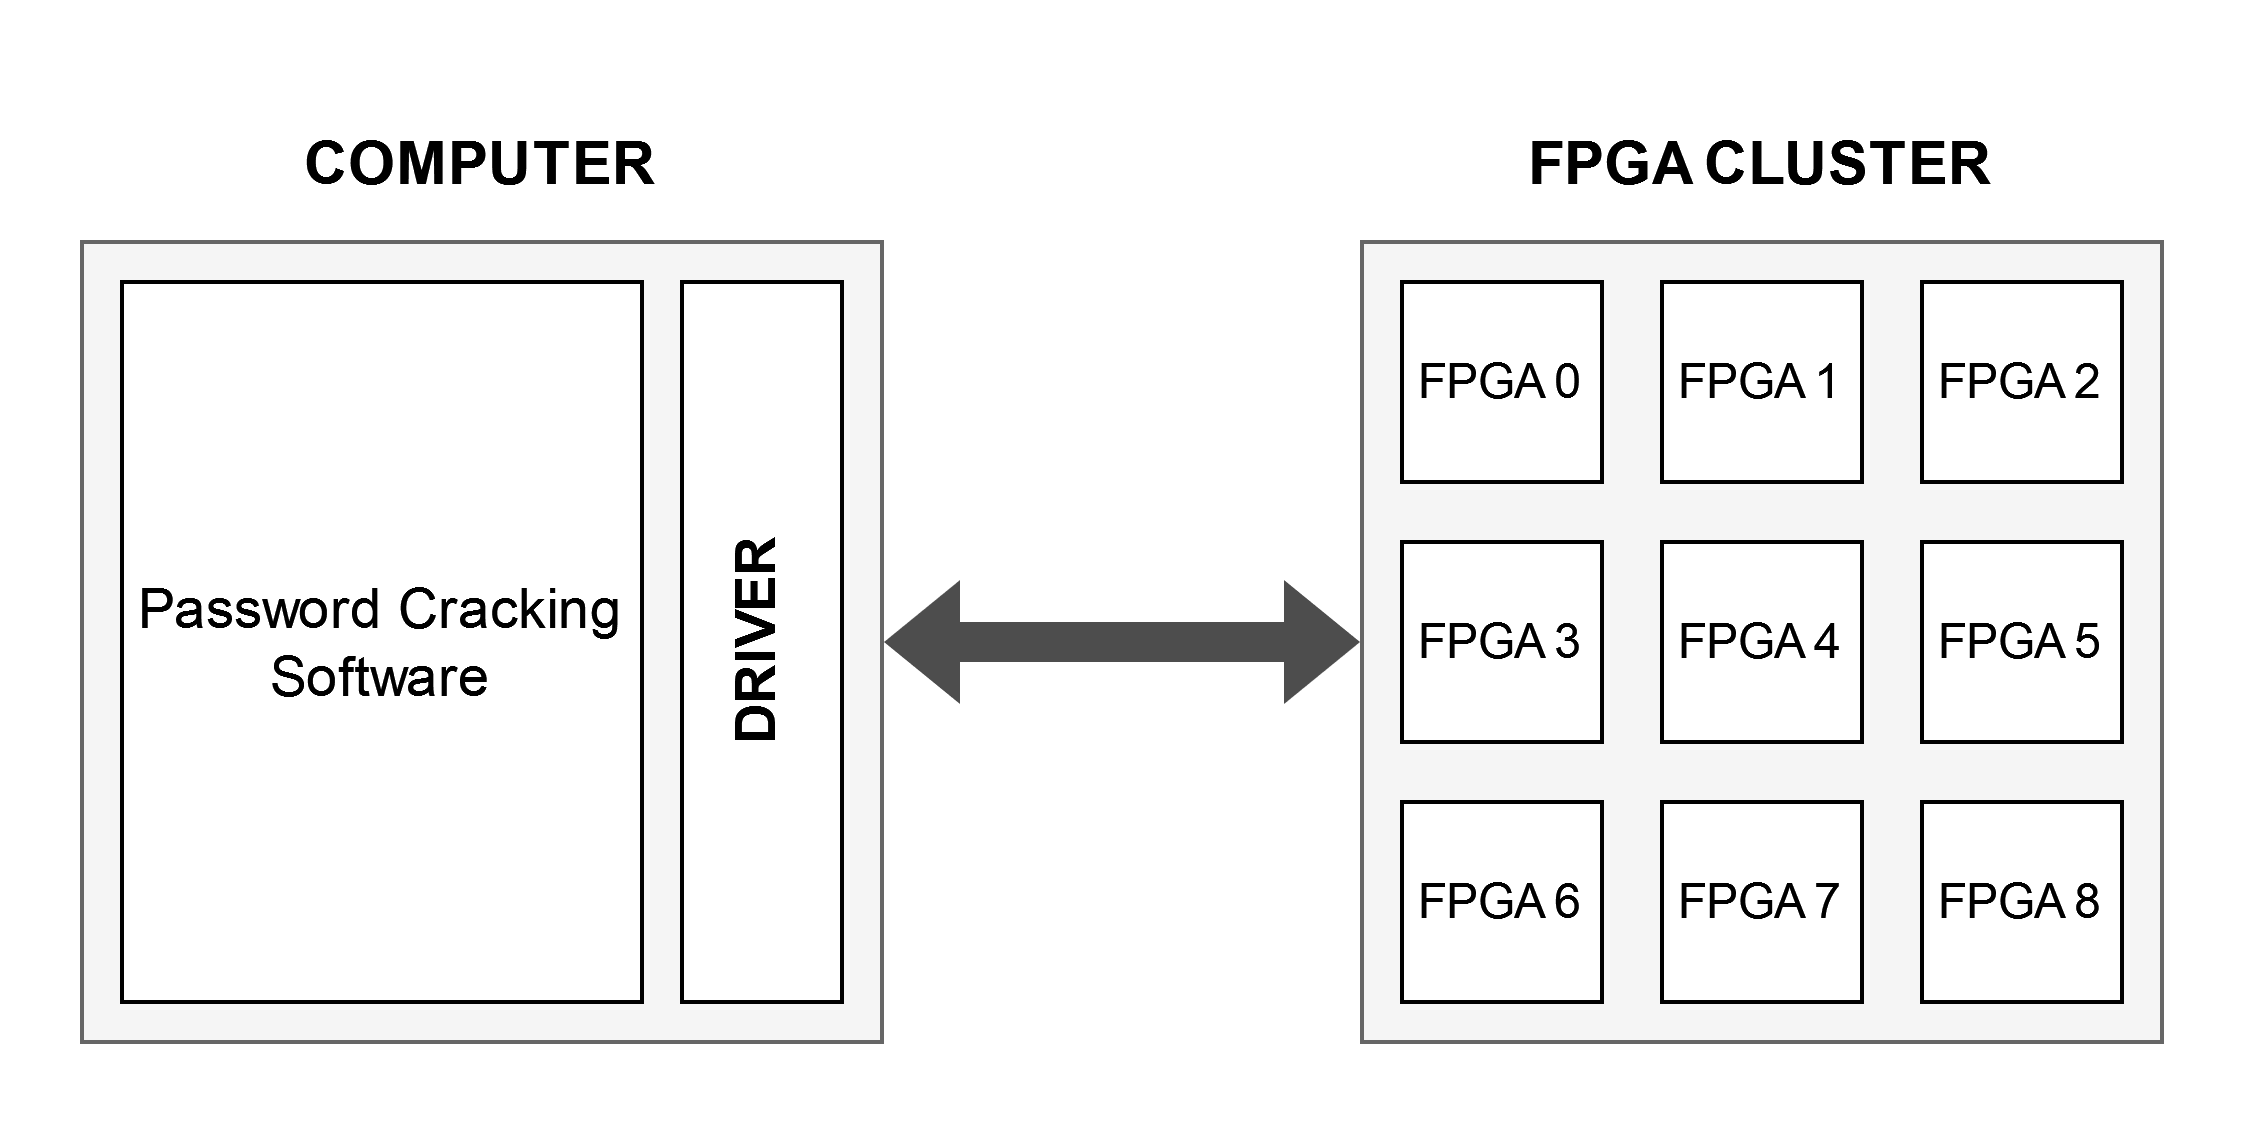
\includegraphics[width=0.9\linewidth]{objectif}
	\caption[Diagramme général]{Diagramme général. Source : réalisé par Kandiah Abivarman}
	\label{fig:objectif}
\end{figure}

Une des première question qu'on s'était posée avec mes professeurs responsables était la manière pour générer les mots de passe lors d'une attaque. 
Dans notre cas, nous avions deux possibilités, soit nous générons les mots de passe directement depuis le \gls{pc} et devons les transmettre à la carte \gls{fpga} afin de procéder au hachage, soit la génération se fait directement dans le \gls{fpga}. 
La différence est que dans le premier cas, on peut être potentiellement limité au niveau logiciel par le \gls{pc} ou au niveau de la communication avec le \gls{fpga}. 
Toutefois, au niveau de la génération des mots de passe, on aura plus de flexibilité permettant d'autres types d'attaques comme par exemple une attaque par dictionnaire\footcite{noauthor_attaque_2021}.

Pour le projet de semestre, j'ai décidé de partir plutôt vers la génération sur \gls{fpga}, afin d'avoir une première solution entièrement fonctionnelle sur \gls{fpga} sans dépendance avec un \gls{pc}. La génération sur \gls{pc} est toutefois envisageable par la suite pour le projet de bachelor.

\section{Bcrypt}

Pour ce projet, nous avons décidé de cibler le Bcrypt, car c'est une fonction de hachage qui prend du temps à être calculé. 

Le Bcrypt est une fonction de hachage avec comme particularité, un paramètre supplémentaire qui est le cost (coût en français).
Ce paramètre va définir le nombre d'itérations que va prendre la fonction de hachage, de ce fait plus le cost est élevé, plus le calcul va prendre du temps.

\subsection{Algorithme}

L'algorithme du Bcrypt se base sur l'algorithme de chiffrement Blowfish\footcite{noauthor_blowfish_2019} qui est une fonction de chiffrement à clef symétrique, c'est-à-dire que la même clef est utilisée pour le chiffrement et le déchiffrement. 
L'algorithme du Bcrypt peut être divisé en deux grandes étapes.

On a une première étape qui est une phase de mise en place des clés symétriques. 
Dans cette étape, on va créer les clés de chiffrements à partir des paramètres d'entrée de la fonction de hachage (mot de passe, salt, cost). 
Cette première étape est la partie la plus coûteuse de la fonction, car la mise en place de la clé va prendre plus ou moins de temps en fonction du cost. 
Les clés de chiffrement sont composées de Subkeys qui est un tableau de 18 entiers de 32 bits et quatre \gls{sbox} qui sont chacun des tableaux de 256 entiers de 32 bits. 
Avant de calculer ces clés de chiffrements, ils sont tout d'abord initialisés avec les décimales de PI.

Puis il y a la deuxième étape, où l'on va utiliser les clés de chiffrement qui ont été calculées plus tôt afin de chiffrer la phrase magique "OrpheanBeholderScryDoubt", le chiffrement va être fait 64 fois.

\begin{figure}[tbph!]
	\centering
	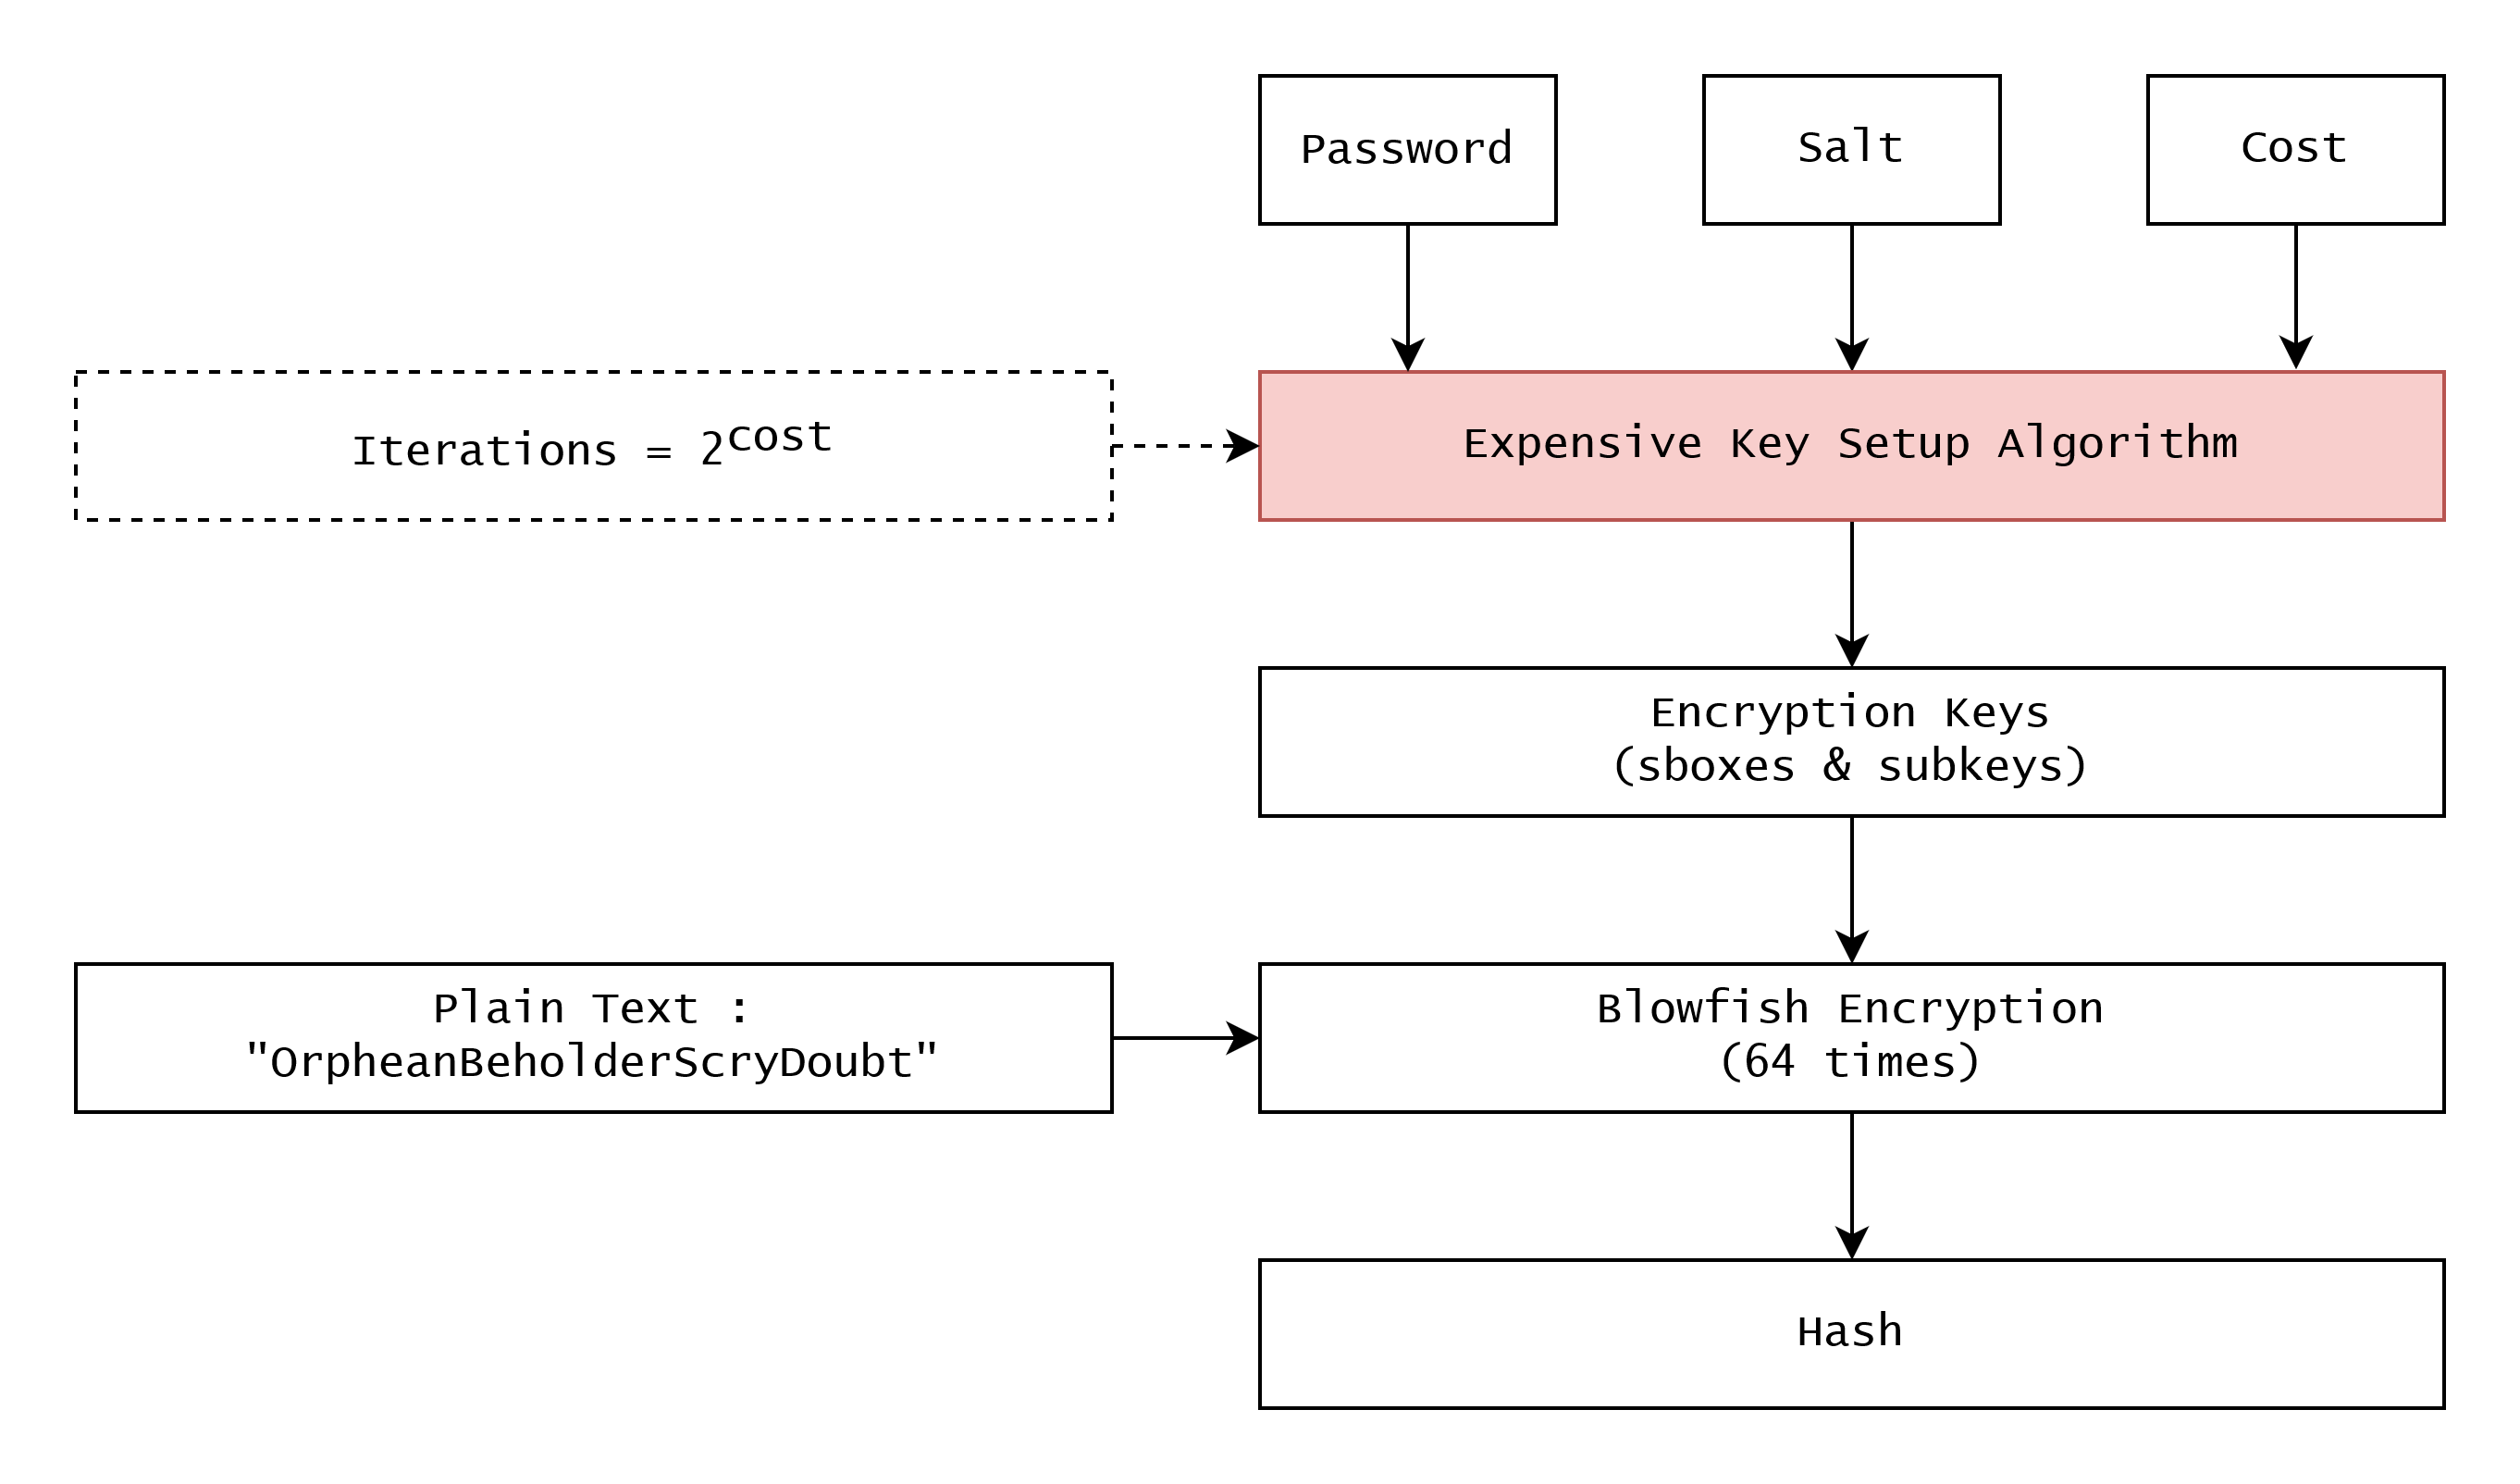
\includegraphics[width=0.9\linewidth]{bcrypt_algo}
	\caption[Algorithme Bcrypt]{Algorithme Bcrypt. Source : réalisé par Kandiah Abivarman}
	\label{fig:bcrypt_algo}
\end{figure}

\subsection{Format du Hash}

Le hash généré par la fonction Bcrypt est généralement stocker sous une forme particulière. 

\begin{figure}[tbph!]
	\centering
	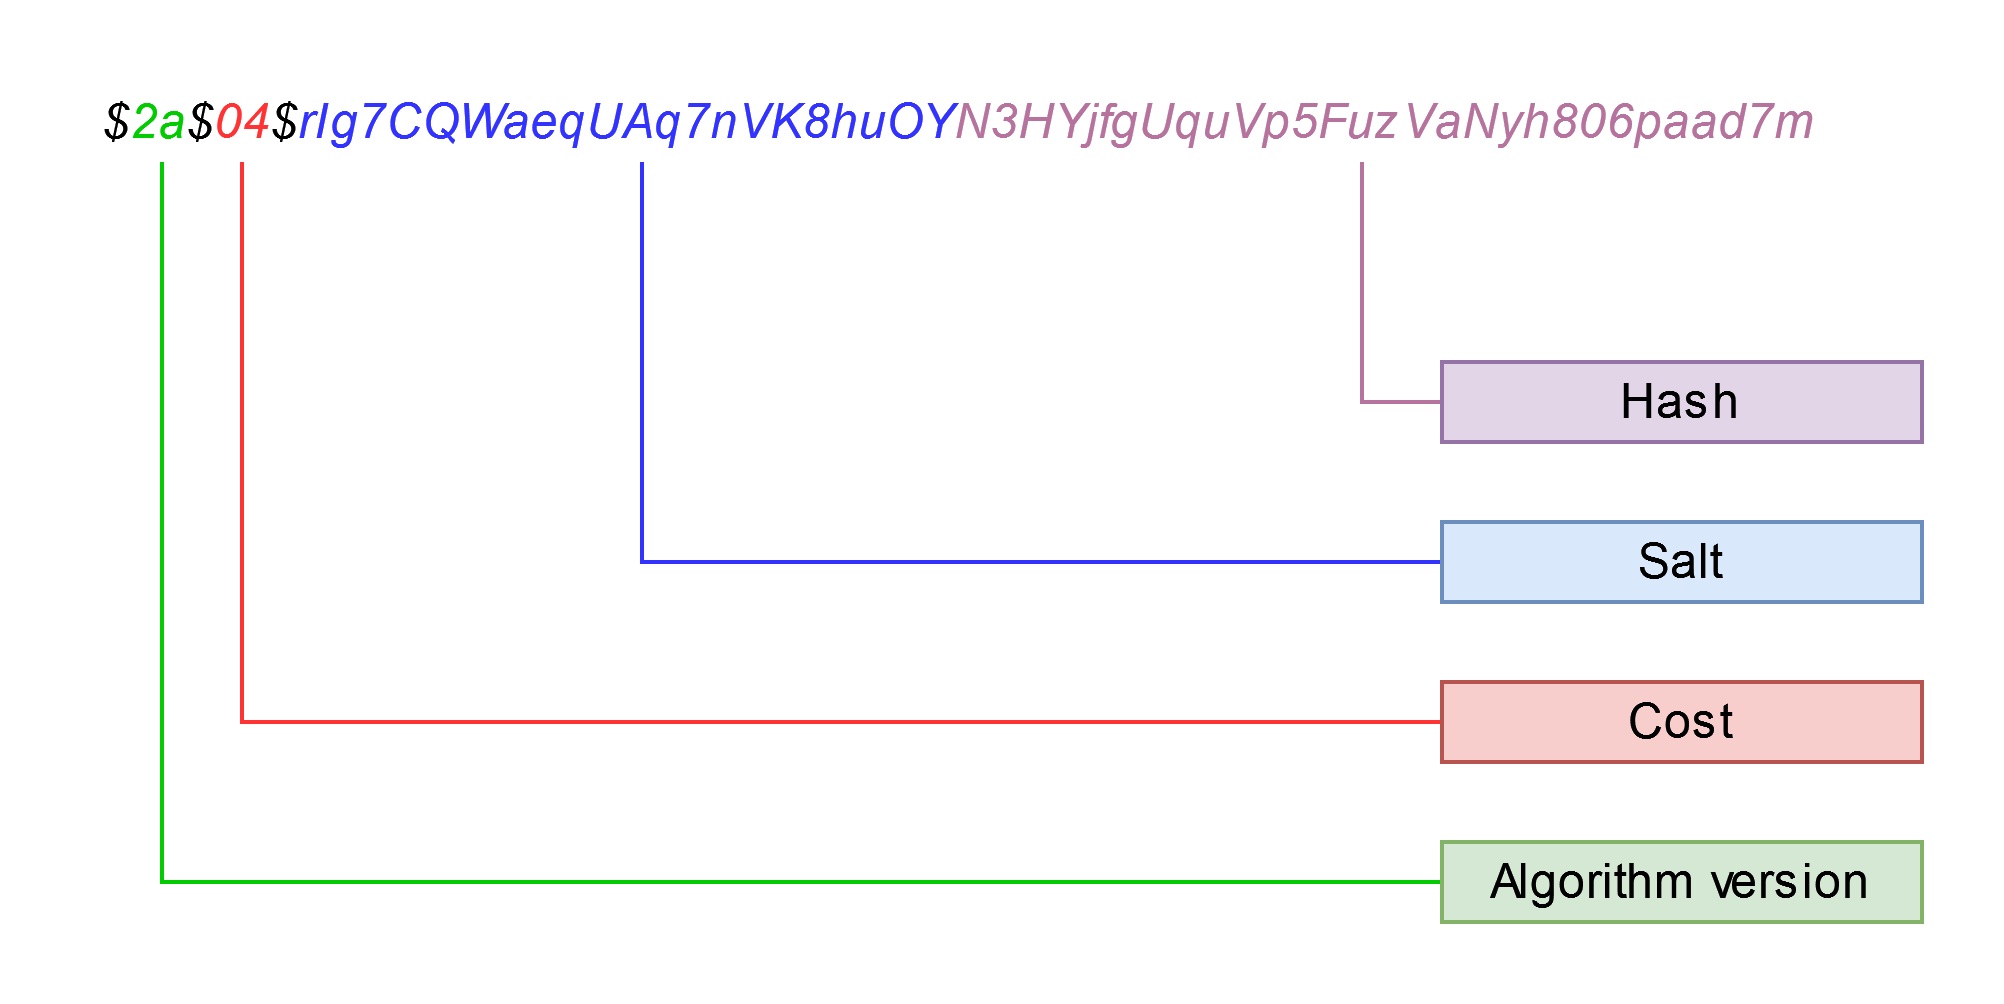
\includegraphics[width=0.9\linewidth]{bcrypt_hash_format}
	\caption[Format du hash Bcrypt]{Format du hash Bcrypt. Source : réalisé par Kandiah Abivarman}
	\label{fig:bcrypt_hash_format}
\end{figure}

On va avoir un premier champ qui contient la version de l'algorithme, un deuxième qui contient le cost de la fonction, un troisième avec le salt et le quatrième avec le hash généré. 
Le salt et le hash sont en base 64, mais il faut faire attention, car c'est une base 64 différente de la norme RFC 4648\footcite{josefsson_base16_2006} qui est couramment utilisé.

\begin{figure}[tbph!]
	\centering
	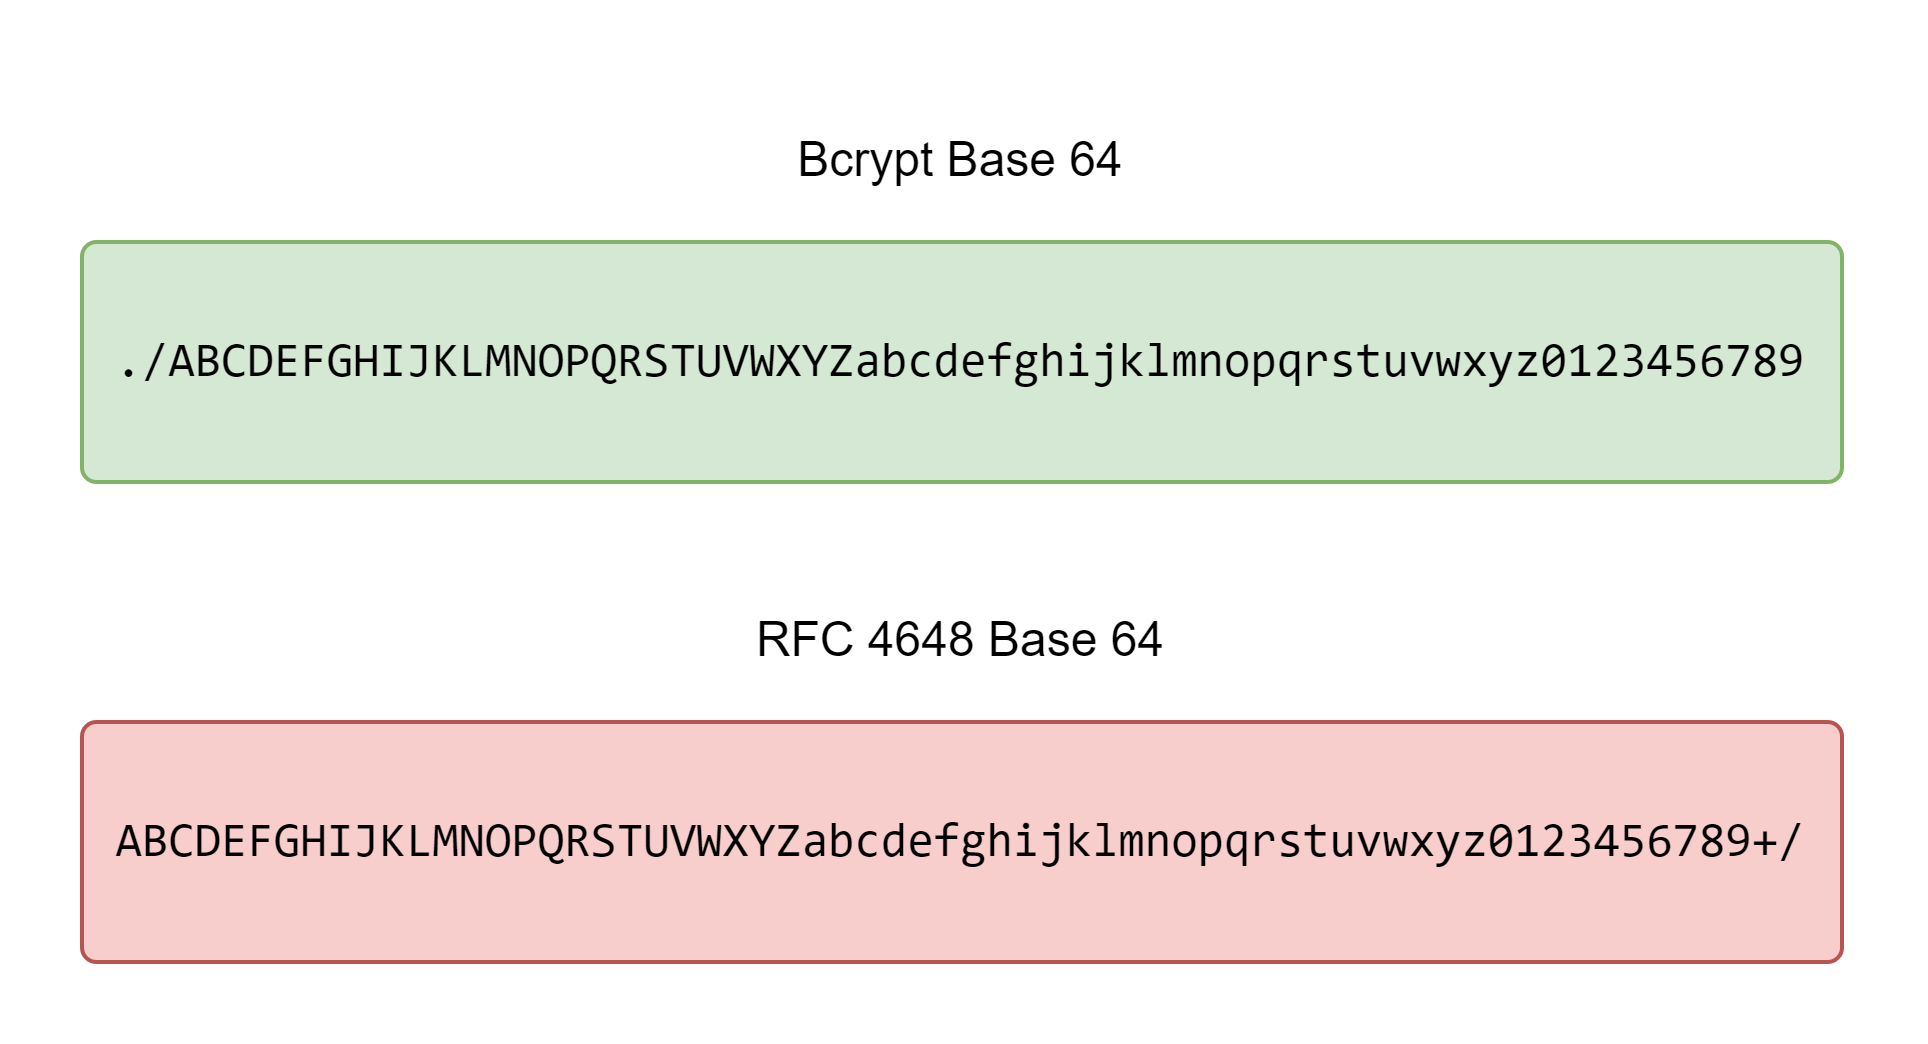
\includegraphics[width=0.9\linewidth]{base_64}
	\caption[Différence Base 64]{Différence Base 64. Source : réalisé par Kandiah Abivarman}
	\label{fig:base_64}
\end{figure}

\section{Implémentations Existantes}

Afin d'éviter de réinventer la roue, la première tâche que j'ai entrepris est de chercher afin de voir s'il n'existe pas déjà des implémentations existantes sur \gls{fpga}. 

D'après mes recherches, j'ai retrouvé seulement deux implémentations du Bcrypt sur FPGA. 
La première se situe dans le répertoire github de JohnTheRipper\footcite{noauthor_openwalljohn_2024} qui est un logiciel de cyber-sécurité destiné au craquage de mot de passe, l'implémentation a été faite en Verilog et spécifiquement pour la Ztex 1.15y qui est une carte FPGA assez ancienne et difficilement retrouvable. 
La deuxième est une implémentation faite en \gls{vhdl} que j'ai aussi retrouvé dans un répertoire github\footcite{noauthor_rub-hgihigh-speed_bcrypt_nodate}, accompagné d'un papier\footcite{wiemer_high-speed_2014} décrivant un travail de recherche effectué sur l'attaque de mot de passe sur FPGA. 
Pour ma part, connaissant seulement le \gls{vhdl} et ne comprenant pas réellement la structure de code du premier et par manque d'informations, j'ai préféré reprendre le code du deuxième. 

Le papier venant avec le code source a été très instructif, j'ai pu notamment comprendre les différents choix qui ont été pris dans le code source. 
Malheureusement, tout n'a pas été documenté et le répertoire n'a pas été mis en place correctement. 
En effet, certains partie du code contenait pas mal d'erreur, des fichiers de tests étaient incomplets et des fichiers source semble avoir été retravaillé en aval.
Au final la plupart des fichiers de tests qui ont été fournis n'était plus utilisables.